\documentclass[12pt,a4paper,oneside]{article}

\usepackage[utf8]{inputenc}
\usepackage[portuguese]{babel}
\usepackage[T1]{fontenc}
\usepackage{amsmath}
\usepackage{amsfonts}
\usepackage{amssymb}
\usepackage{graphicx}

\usepackage{xcolor}
% Definindo novas cores
\definecolor{verde}{rgb}{0.25,0.5,0.35}
\definecolor{jpurple}{rgb}{0.5,0,0.35}
% Configurando layout para mostrar codigos Java
\usepackage{listings}
\lstset{
  language=Java,
  basicstyle=\ttfamily\small, 
  keywordstyle=\color{jpurple}\bfseries,
  stringstyle=\color{red},
  commentstyle=\color{verde},
  morecomment=[s][\color{blue}]{/**}{*/},
  extendedchars=true, 
  showspaces=false, 
  showstringspaces=false, 
  numbers=left,
  numberstyle=\tiny,
  breaklines=true, 
  backgroundcolor=\color{cyan!10}, 
  breakautoindent=true, 
  captionpos=b,
  xleftmargin=0pt,
  tabsize=4,
  escapeinside=||
}

\author{\\Universidade Federal de Goiás (UFG) - Regional Jataí\\Bacharelado em Ciência da Computação \\Inteligência Artificial \\Esdras Lins Bispo Jr.}

\title{\sc \huge Primeira Prova \\(Segunda Chamada)}

\begin{document}

\maketitle

{\bf ORIENTAÇÕES PARA A RESOLUÇÃO}

\begin{itemize}
	\item A avaliação é individual, sem consulta;
	\item A pontuação máxima desta avaliação é 10,0 (dez) pontos, sendo uma das 04 (quatro) componentes que formarão a média final da disciplina: duas provas, um projeto e exercícios;
	\item A média final será calculada pela média ponderada das quatro supraditas notas [em que a primeira prova tem peso 35 (trinta e cinco), a segunda prova tem peso 25 (vinte e cinco), o projeto tem peso 30 (trinta) e os exercícios têm peso 10 (dez)];
	\item O somatório da pontuação de todas as questões desta avaliação é 11,0 (onze) pontos. Isto é um sinônimo de tolerância na correção. Se você por acaso perder 1,5 (um e meio), sua nota será 9,5 (nove e meio);
	\item O conteúdo exigido compreende os seguintes pontos apresentados no Plano de Ensino da disciplina: (1) Introdução à Inteligência Artificial, (2) Agentes Inteligentes, (3) Resolução de Problemas, (7) Aprendizado de Máquina e (8) Mineração de dados.
\end{itemize}

\begin{center}
	\fbox{\large Nome: \hspace{10cm}}
	\fbox{\large Assinatura: \hspace{9cm}}
\end{center}

\newpage

\begin{enumerate}

	\item (2,0 pt) Descreva duas das quatro definições de Inteligência Artificial apresentadas em sala de aula.
	
	\item (2,0 pt) Em um labirinto, mostrado na figura a seguir, um robô é colocado na célula inicial indicada por ``E'' e deve encontrar um caminho até a saída, denotada pela letra ``S''. O robô não pode se mover na diagonal, somente acima, abaixo, direita e esquerda. Ele também não pode atravessar paredes (as linhas mais grossas da grade) ou as bordas do labirinto, de modo que ele é forçado a contornar obstáculos. Felizmente, o robô possui um mapa do ambiente. A solução é o caminho mais curto até a saída e todos os movimentos do robô possuem os mesmos custos.	
	
	\begin{center}
		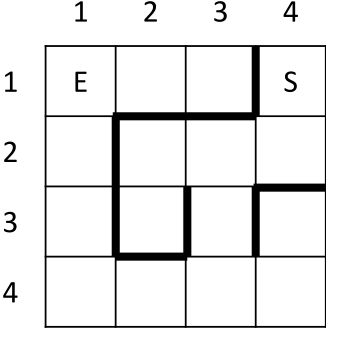
\includegraphics[width=5cm]{images/fig03.png}
	\end{center}		
	
	\begin{enumerate}
		\item Descreva o problema em termos de um problema de busca definindo o espaço de estados, o estado inicial, o estado final, os operadores de transição entre os estados (ações) e o custo.
	\end{enumerate}
	
	\item (3,0 pt) Considere um espaço de estados em que o estado inicial é o número 1 e a função sucessor para o estado $n$ retorna dois estados, com números $2(n+1)$ e $2(n+1)+1$.

		\begin{enumerate}
			\item (1,0 pt) Desenhe a porção do espaço de estados correspondente aos estados entre 1 e 17.
			\item (2,0 pt) Suponha que o estado objetivo seja 13. Liste a ordem em que os nós serão visitados no caso da busca em extensão (largura) e a busca por aprofundamento iterativo.
		\end{enumerate}
	
	\newpage
	
	\item (4,0 pt) Construa o índice invertido (conforme apresentado em sala de aula) para a coleção de documentos abaixo:
		
		\begin{itemize}
			\item[] {\bf Doc1} \ \ disciplina de logica matematica
			\item[] {\bf Doc2} \ \ logica para ciencia da computacao
			\item[] {\bf Doc3} \ \ inteligencia artificial com programacao logica
			\item[] {\bf Doc4} \ \ matematica computacional
		\end{itemize}
	
	\end{enumerate}
\end{document}